\section{Durchführung}
\label{sec:Durchführung}

Um die effektive Masse der Elektronen bestimmen zu können, muss sichergestellt werden,
dass lediglich die Faraday-Rotation betrachtet wird. Deshalb wird ebenfalls eine Messung
mit reinem GaAs durchgeführt, um später die Differenz aus beiden Rotationen zu bilden.

\subsection{Versuchsaufbau}

Der Versuchsaufbau ist in \autoref{fig:Aufbau} dargestellt und wird im folgenden genauer erläutert.

\begin{figure} [H]
    \centering
    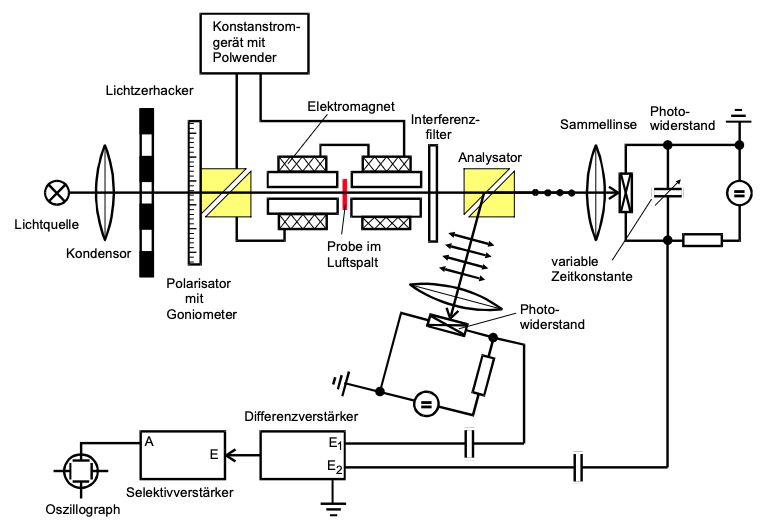
\includegraphics[height=8cm]{content/Aufbau.png}
    \caption{Versuchsaufbau inklusive aller Messapperaturen. \cite{V46}}
    \label{fig:Aufbau}
\end{figure}

Eine Halogenlampe dient als Lichtquelle, sie leuchtet größtenteils im Infrarotbereich, da die Probe für diese Wellenlängen
am durchlässigsten ist. Dannach wird das Licht durch eine Linse gebündelt und mithilfe eines Lichtzerhackers mit einer bekannten
Frequenz von $\qty{450}{\Hz}$ in Pulse geteilt. Mithilfe des darauf folgenden Glan-Thompson-Prismas wird das Licht linear polarisiert.
Das Prisma ist dabei drehbar an einem Goniometer befestigt, sodass die genaue Polarisationsrichtung eingestellt und abgelesen werden kann.
Anschließend wird das Strahlenbündel durch einen Elektromagneten geschickt, in dessen Mitte sich die Probe befindet.
Somit liegt die Probe im Bereich des maximalen B-Feldes, und während das Licht diese durchquert, tritt der in \autoref{sec:Faraday}
beschriebene Faraday-Effekt auf.

Nach dem Magneten ist ein Interferenzfilter platziert, sodass jeweils nur eine Wellenlänge betrachtet werden kann. Das Licht trifft dannach auf
einen Analysator, der den Strahl in zwei Teile spaltet, die eine zueinander orthogonale Polarisation besitzen. Beide Strahlen treffen
auf Photoelemente, die daraufhin eine Wechselspannung erzeugen, die ausgekoppelt wird. Beide Spannungen werden mithilfe eines Differenzverstärkers
zusammengeführt, und anschließend in einen Selektivverstärker geführt. Dieser wird auf die Frequenz des Lichtzerhackers abgestimmt, somit kann ein
Großteil des Signalrauschens unterdrückt werden, man bezeichnet dieses Vorgehen auch als Wechsellichtmethode.
Zuletzt wird das Signal des Selektivverstärkers mithilfe eines Oszilloskops visualisiert, sodass eine Amplitude abgelesen werden kann.

\subsection{Versuchsdurchführung}

Als Erstes wird mithilfe einer Hall-Sonde das B-Feld innerhalb der Spule vermessen. Dafür wird die Sonde schrittweise in den Magneten hereingeführt
und es werden Wertepaare aus Abstand und Feldstärke notiert, sodass daraus das Maximum des Feldes ermittelt werden kann.

Bevor die eigentliche Messung beginnt, wird der Strahlengang kontrolliert und justiert um sicherzustellen, dass beide Photoelemente genug Lichtintensität
abbekommen.

Für den Versuch stehen drei GaAs Proben zur Verfügung, von denen eine undotiert ist, diese wird zuerst in der Mitte des Magneten platziert.
Um den Rotationswinkel zu messen, wird der Winkel des Glan-Thompson-Prismas
solange verstellt, bis das Signal am Oszilloskop ein Minimum annimmt. Es wird nun der entsprechende Winkel am Goniometer abgelesen und
die Prozedur mit umgepolten B-Feld wiederholt. Diese Messung wird mit 9 verschiedenen Interferenzfiltern durchgeführt, um genug unterschiedliche Wellenlängen für einen
Fit in der Auswertung zur Verfügung zu haben.
Zuletzt wird die Messung zwei weitere Male mit den dotiertem GaAs Proben durchgeführt.